% Native editable composition from verified, unchanged IDE images.
\par
\begin{figure}[htbp]
  \centering
  \sbox0{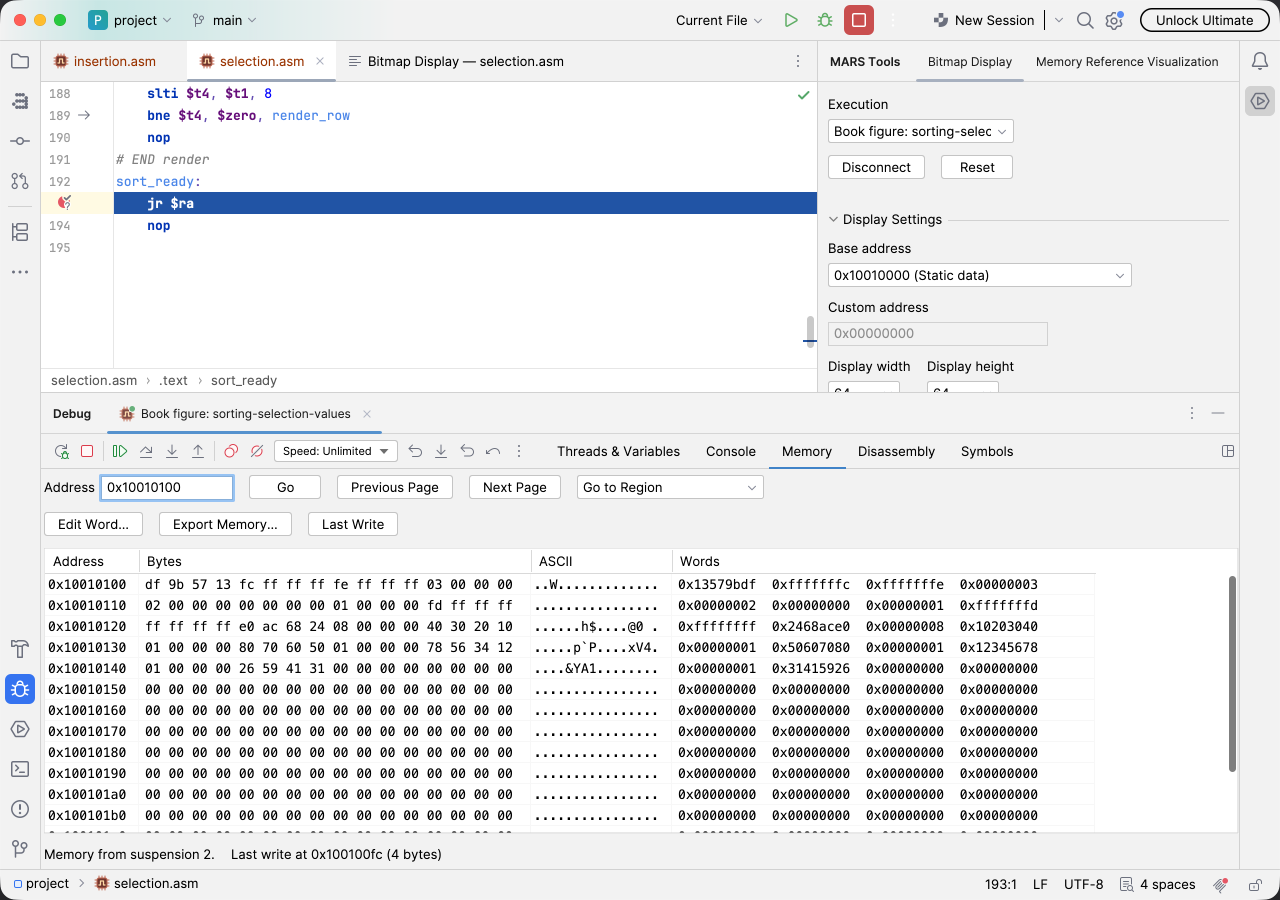
\includegraphics[artifact]{packages/009-sorting-visualizer/captures/f03-selection/values.png}}
  \sbox2{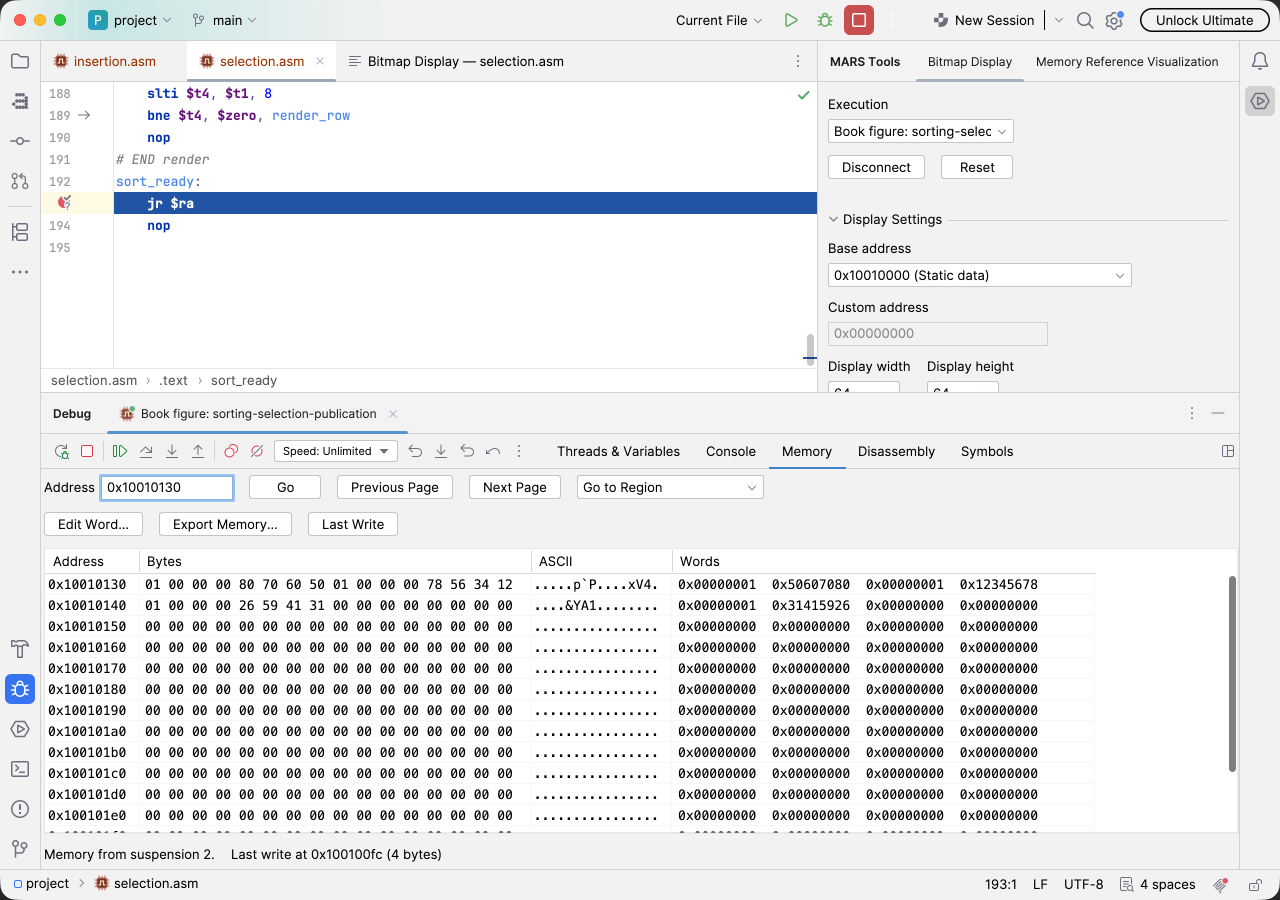
\includegraphics[artifact]{packages/009-sorting-visualizer/captures/f03-selection/publication.png}}
  \sbox4{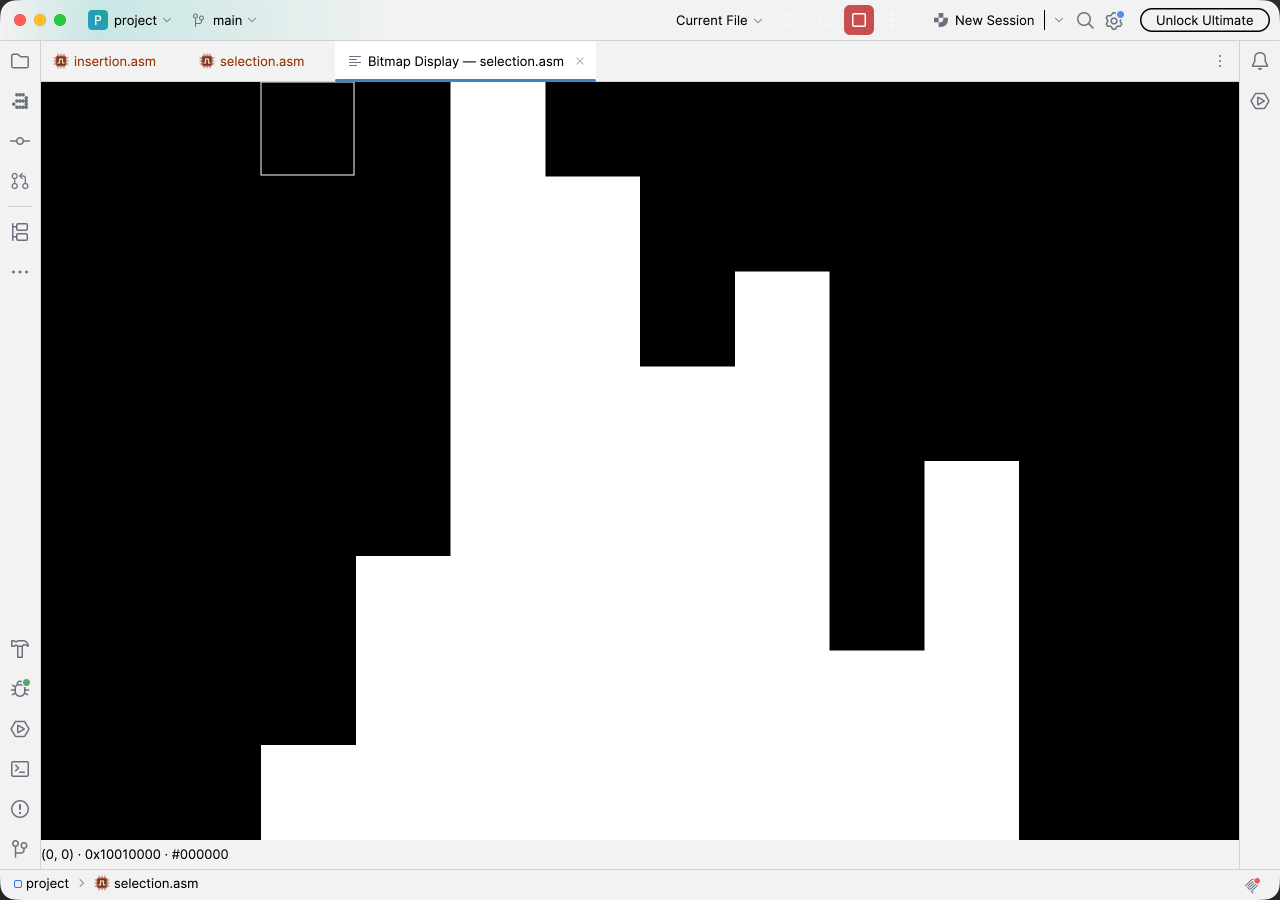
\includegraphics[artifact]{packages/009-sorting-visualizer/captures/f03-selection/bitmap.png}}
  \edef\MARSselectionsourceLeft{\the\dimexpr0.036718750\wd0\relax}
  \edef\MARSselectionsourceBottom{\the\dimexpr0.757777778\ht0\relax}
  \edef\MARSselectionsourceRight{\the\dimexpr0.611718750\wd0\relax}
  \edef\MARSselectionsourceTop{\the\dimexpr0.164444444\ht0\relax}
  \edef\MARSselectionstateLeft{\the\dimexpr0.034375000\wd0\relax}
  \edef\MARSselectionstateBottom{\the\dimexpr0.287777778\ht0\relax}
  \edef\MARSselectionstateRight{\the\dimexpr0.578906250\wd0\relax}
  \edef\MARSselectionstateTop{\the\dimexpr0.608888889\ht0\relax}
  \edef\MARSselectionmemoryLeft{\the\dimexpr0.034375000\wd2\relax}
  \edef\MARSselectionmemoryBottom{\the\dimexpr0.311111111\ht2\relax}
  \edef\MARSselectionmemoryRight{\the\dimexpr0.578906250\wd2\relax}
  \edef\MARSselectionmemoryTop{\the\dimexpr0.608888889\ht2\relax}
  \edef\MARSselectionplotLeft{\the\dimexpr0.203906250\wd4\relax}
  \edef\MARSselectionplotBottom{\the\dimexpr0.066666667\ht4\relax}
  \edef\MARSselectionplotRight{\the\dimexpr0.203906250\wd4\relax}
  \edef\MARSselectionplotTop{\the\dimexpr0.091111111\ht4\relax}
  \begin{tikzpicture}[alt={Four annotated details after the first selection exchange. The signed array is minus four, minus two, three, two, zero, one, minus three, minus one. The algorithm selector is one, phase is one and exchange count is one. Columns zero and three now have heights one and seven. Instruction text is identical to the insertion fixture.}]
    \node[anchor=north west,inner sep=0,font=\small\bfseries] (source-title) at (6mm,0) {Next instruction: return from the renderer};
    \node[anchor=north west,inner sep=0] (source) at ([yshift=-1mm]source-title.south west) {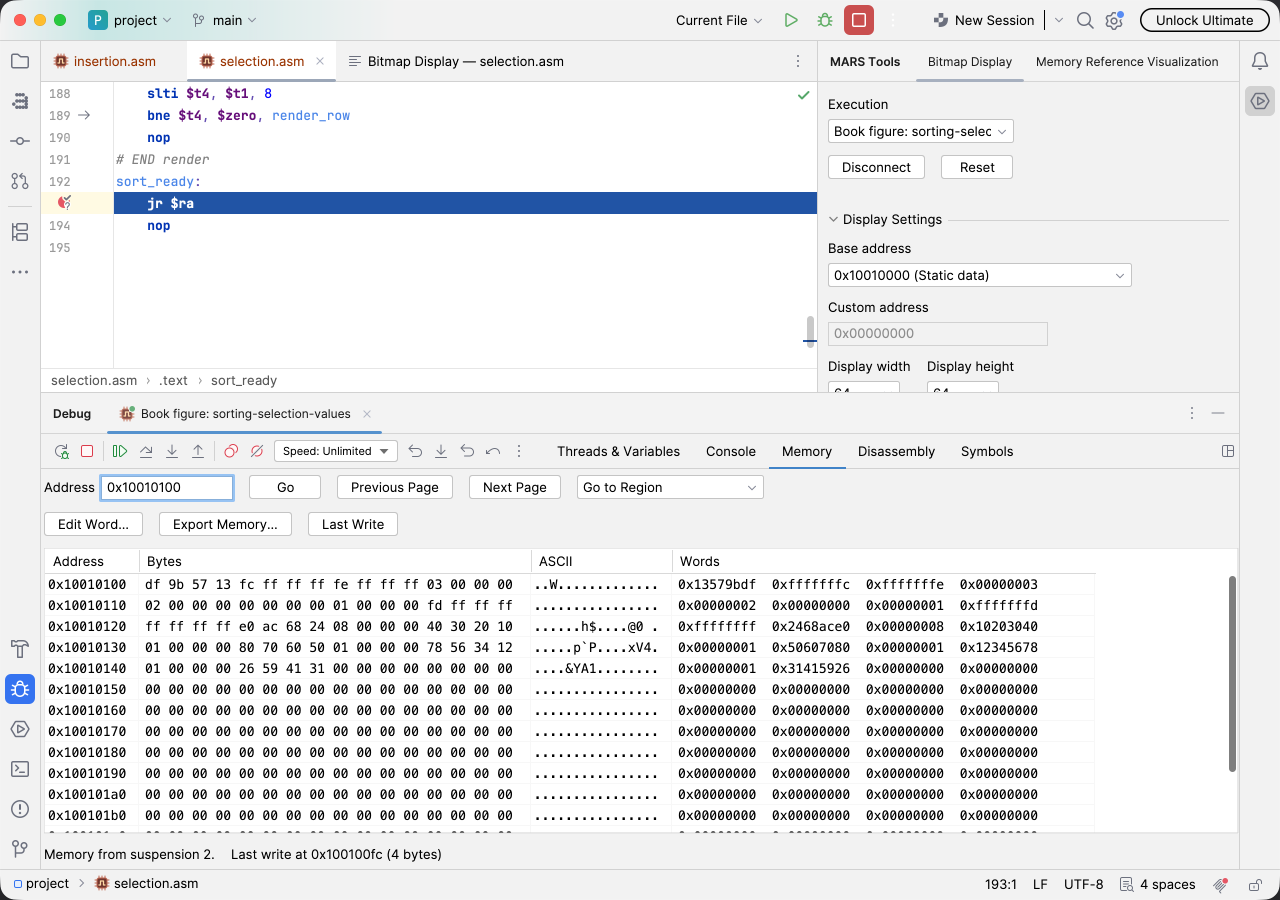
\includegraphics[width=0.7\linewidth,artifact,trim={\MARSselectionsourceLeft{} \MARSselectionsourceBottom{} \MARSselectionsourceRight{} \MARSselectionsourceTop{}},clip]{packages/009-sorting-visualizer/captures/f03-selection/values.png}};
    \begin{scope}[shift={(source.south west)},x={($(source.south east)-(source.south west)$)},y={($(source.north west)-(source.south west)$)}]
      \draw[black,line width=0.7pt] (0.153333333,0.057142857) rectangle (0.326666667,0.371428571);
      \node[draw=black,fill=white,circle,inner sep=1.5pt,font=\footnotesize] at ($(0.153333333,0.371428571)+(-3mm,0)$) {1};
    \end{scope}
    \node[anchor=north west,inner sep=0,font=\small\bfseries] (state-title) at ([yshift=-1mm]source.south west) {Signed array words and neighboring guards};
    \node[anchor=north west,inner sep=0] (state) at ([yshift=-1mm]state-title.south west) {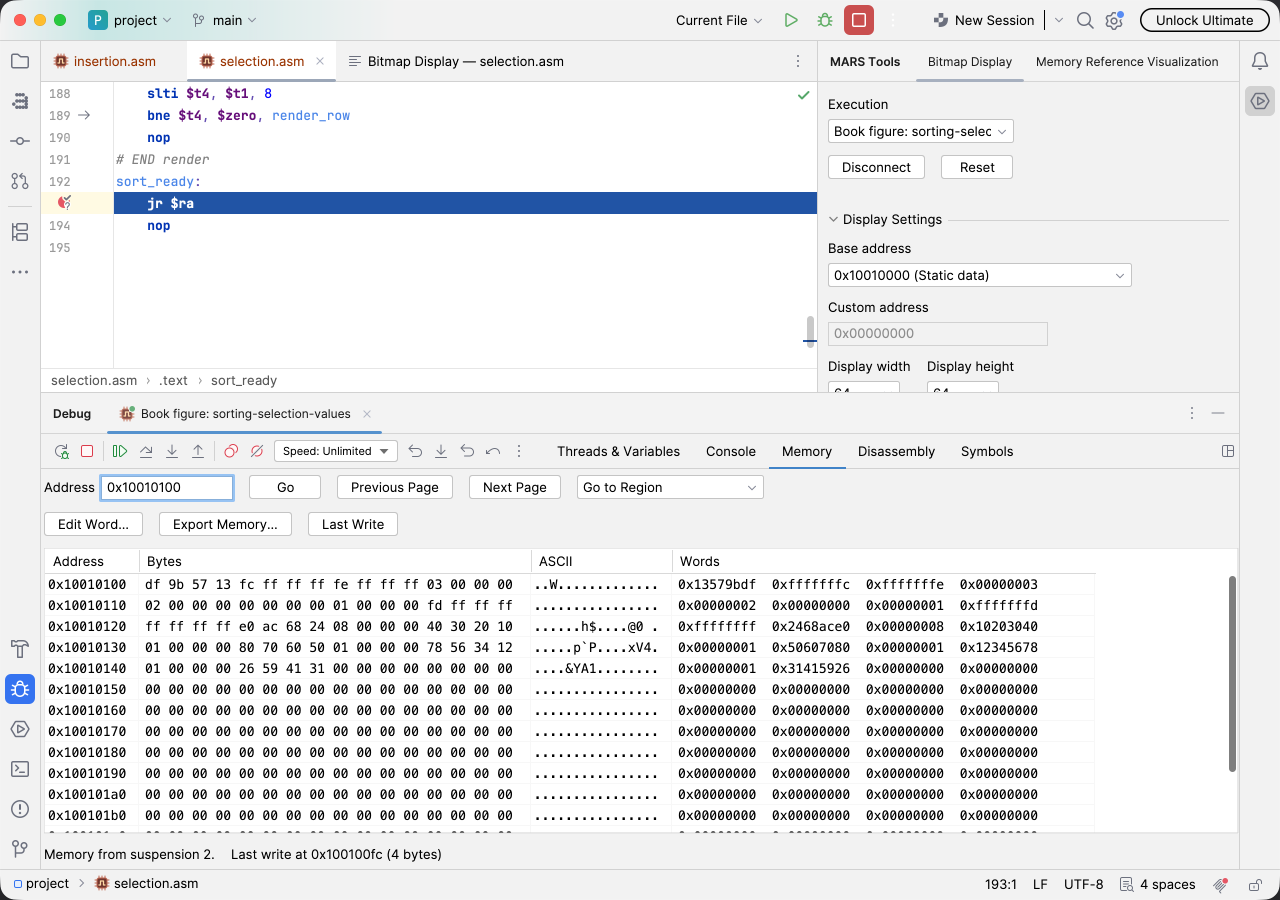
\includegraphics[width=0.78\linewidth,artifact,trim={\MARSselectionstateLeft{} \MARSselectionstateBottom{} \MARSselectionstateRight{} \MARSselectionstateTop{}},clip]{packages/009-sorting-visualizer/captures/f03-selection/values.png}};
    \begin{scope}[shift={(state.south west)},x={($(state.south east)-(state.south west)$)},y={($(state.north west)-(state.south west)$)}]
      \draw[black,line width=0.7pt] (0.191919192,0.043010753) rectangle (0.983838384,0.720430108);
      \node[draw=black,fill=white,circle,inner sep=1.5pt,font=\footnotesize] at ($(0.191919192,0.720430108)+(-3mm,0)$) {2};
    \end{scope}
    \node[anchor=north west,inner sep=0,font=\small\bfseries] (memory-title) at ([yshift=-1mm]state.south west) {Algorithm, phase and completed-exchange count};
    \node[anchor=north west,inner sep=0] (memory) at ([yshift=-1mm]memory-title.south west) {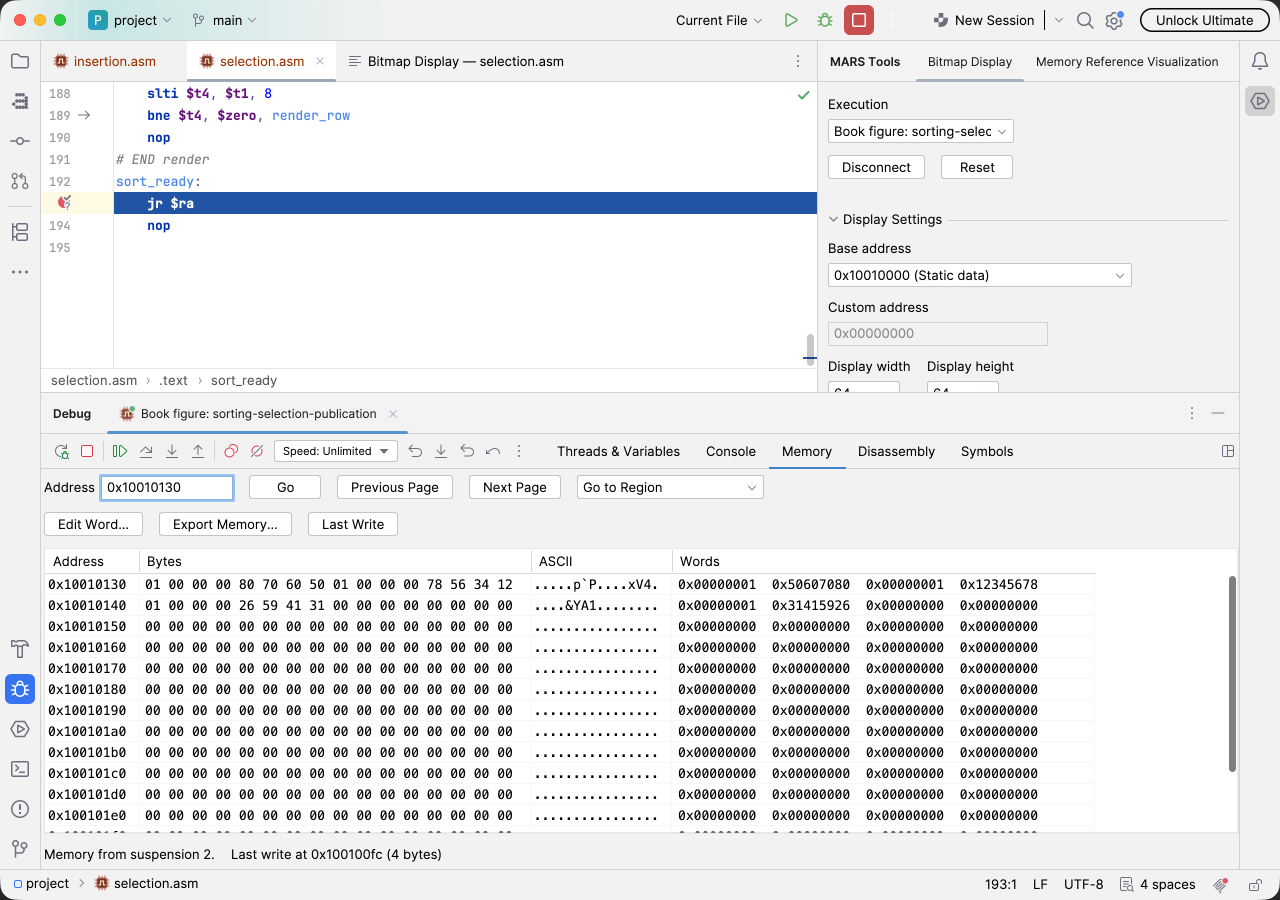
\includegraphics[width=0.78\linewidth,artifact,trim={\MARSselectionmemoryLeft{} \MARSselectionmemoryBottom{} \MARSselectionmemoryRight{} \MARSselectionmemoryTop{}},clip]{packages/009-sorting-visualizer/captures/f03-selection/publication.png}};
    \begin{scope}[shift={(memory.south west)},x={($(memory.south east)-(memory.south west)$)},y={($(memory.north west)-(memory.south west)$)}]
      \draw[black,line width=0.7pt] (0.191919192,0.055555556) rectangle (0.983838384,0.638888889);
      \node[draw=black,fill=white,circle,inner sep=1.5pt,font=\footnotesize] at ($(0.191919192,0.638888889)+(-3mm,0)$) {3};
    \end{scope}
    \node[anchor=north west,inner sep=0,font=\small\bfseries] (plot-title) at ([yshift=-1mm]memory.south west) {Complete published framebuffer};
    \node[anchor=north west,inner sep=0] (plot) at ([yshift=-1mm]plot-title.south west) {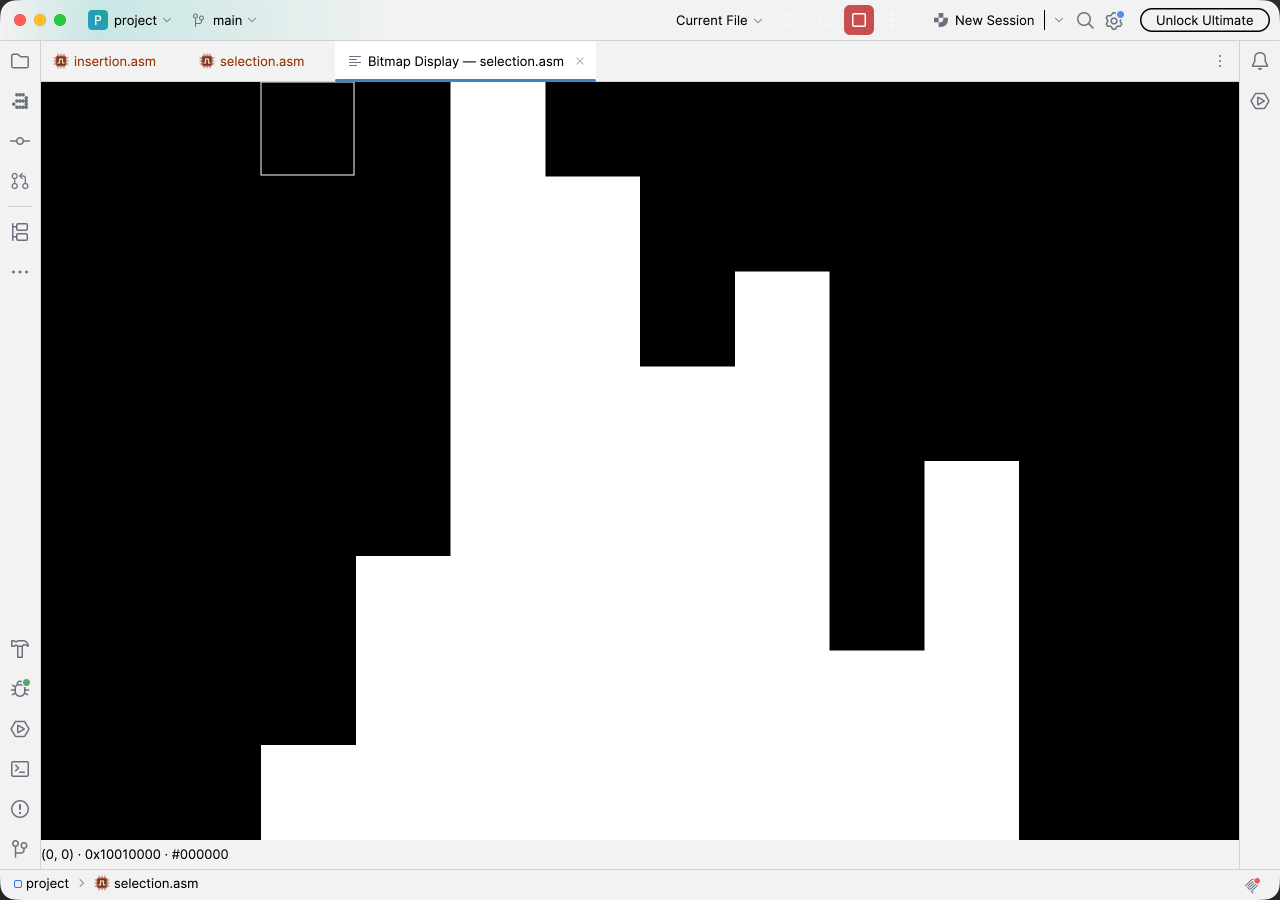
\includegraphics[width=0.24\linewidth,artifact,trim={\MARSselectionplotLeft{} \MARSselectionplotBottom{} \MARSselectionplotRight{} \MARSselectionplotTop{}},clip]{packages/009-sorting-visualizer/captures/f03-selection/bitmap.png}};
    \begin{scope}[shift={(plot.south west)},x={($(plot.south east)-(plot.south west)$)},y={($(plot.north west)-(plot.south west)$)}]
      \draw[black,line width=0.7pt] (0.000000000,0.000000000) rectangle (1.000000000,1.000000000);
      \node[draw=black,fill=white,circle,inner sep=1.5pt,font=\footnotesize] at ($(0.000000000,1.000000000)+(-3mm,0)$) {4};
      \foreach \c in {0,...,7} {\node[anchor=north,font=\scriptsize,inner sep=0] at ({(\c+0.5)/8},-0.035) {\c}; \node[anchor=east,font=\scriptsize,inner sep=0] at (-0.025,{1-(\c+0.5)/8}) {\c};}
      \node[anchor=north,font=\scriptsize,inner sep=0] at (0.5,-0.11) {$x$}; \node[anchor=east,font=\scriptsize,inner sep=0] at (-0.10,0.5) {$y$};
    \end{scope}
  \end{tikzpicture}
  \par\smallskip
  \begin{minipage}{\linewidth}
    \small
    \begin{enumerate}
      \item This separate execution uses selector 1 and the native condition \texttt{\$s6 == 1}. The same \texttt{sort\_ready} instruction is reached after a selection-sort redraw. The program instructions are identical; only the documented selector word differs between fixtures.
      \item The array is $[-4,-2,3,2,0,1,-3,-1]$. The minimum of the initial suffix is $-4$ at index 3. Selection exchanges that word with 2 at index 0. It does not move $-4$ through each intervening position; values at indices 1 and 2 stay in place.
      \item The selector bytes are \texttt{01 00 00 00}. Phase 1 and exchange count 1 follow the same completed-exchange protocol as insertion sort. Equal counts here describe different exchanges: adjacent indices 0 and 1 for insertion, but indices 0 and 3 for selection.
      \item Column 0 has one white cell at row 7, and column 3 has seven beginning at row 1. Their new heights encode $-4$ and 2. All other columns match the initial frame. Signed comparison matters: the most negative value is the shortest bar under this offset encoding.
    \end{enumerate}
  \end{minipage}
  \caption{Selection sort exchanges the suffix minimum with the first position.}
  \label{capture:009-sorting-visualizer-f03-selection}
\end{figure}
\par
